\documentclass[a4paper,11pt]{article}
%在此可进行页面设置
%\textwidth=14cm
%\textheight=22cm

\usepackage[46038]{MCMPackage}  %队号在这里填写
%\usepackage[XXX,nosheet]{MCMPackage}%这个参数形式可去掉summary sheet首页。
\problem{C}  %选题

\title{An Investment in Education is an Investment in The Future}%在此插入论文标题
\date{}

%设置段落之间的距离,若不需要删除或者注释掉即可。
\setlength\parskip{.5\baselineskip}

%为了首行缩进
%\usepackage{indentfirst}
%\setlength{\parindent}{2em}

\begin{document}
%摘要
\begin{abstract}
\par The famous '80-20' rule states that the 80\% influence is caused by the 20\% for many events. This principle is also suitable for the investment. In order to determine an optimal investment strategy, the problem is divided into three requirements and the Optimal Educational Investment Model is proposed to solve it.
\par For the first requirement, we gain Prioritized Candidate List through Return on Investment (ROI). To get more complete data, Support Vector Machine (SVM) is used for data processing. Based on Large Margin Nearest Neighbor (LMNN) method and the '80-20' Rule, we can get the weights of "the graduation rate", "Proportion of students' wages over 25000 dollars after 6 years", "The median income after 10 years" and "Repayment rate of 3 years", which are used to calculate the Return Index(RI). We define ROI as RI divided by the corresponding investment. ROI determines the priority of the investment, and thus the Prioritized Candidate List is obtained. The list shows that Southern Virginia University, Southern Wesleyan University and Lakeland Community College are three most worthy investment universities. 
 \par For the second requirement, based on the relationship between the amount of investment and RI of each universities, we gain a one year optimal investment strategy. According to the "80-20" rule, we invest only 20\% of colleges. In order to ensure the diversity of investment, we set the upper and lower bounds on the proportion of investment funds. To maximize the total RI of each college, we take the limitation of funds as a constraint and build a linear program model. By solving linear programming, we obtain the amount of investment in each college in one year. The result shows we ought to invest 1,040,000 dollars to Southern Virginia University.
\par For the third requirement, we introduced the elimination mechanism to improve the efficiency of investment funds. After one year investment, the invested universities produce new results. Then, we use the first requirement's method to compute the ROI, make a rank, eliminate the last 5\%, and use the second requirement's method to compute the next year's amount of investment. By using the similar method, we can obtain the Prioritized Candidate List of the next 3 years. According to our model, MIT university is not invested in the second year.
\par In order to further study the problem, combined with Reinforcement Learning, Reinforcement Learning Model is established. Compared with the optimal investment model we analyze their respective advantages and disadvantages. Moreover, sensitivity analysis of the upper and lower bounds on the investment and the elimination rate is discussed.

\textbf{Keywords: Support Vector Machine, Large Margin Nearest Neighbor, Linear Program, Return on Investment, Reinforcement Learning}



\end{abstract}
\maketitle%插入标题
\thispagestyle{empty}%本页不遍页码

\newpage%另起一页插入目录
\thispagestyle{empty}%防止目录两页而出现一页带页码
\tableofcontents%目录
\thispagestyle{empty}
\newpage%另起一页书写正文
\pagenumbering{arabic}%开始编页码(阿拉伯数字)

\section{Introduction}
%In reference \cite{RefB}.%引用参考文献

\subsection{Background}
The company faced some managerial problems such as high churn rate, job mismatch, low quality employees and so on. Thus, the \textbf{Human resource (HR)} management is proposed as a suitable proposal to improve the situation. Human resource management is a function in organizations designed to maximize employee performance in service of an employer's strategic objectives. HR is primarily concerned with the management of people within organizations, focusing on policies and systems.

The hired excellent HR specialists need to achieve the following tasks:
\begin{itemize}
    \item Design a robust and well-rounded corporate structure, which match the suitable employees to the right position according to their talents and stays stable when people churn
    \item Arrange the enterprise training and promotion reasonably to provide the elites the chance of ability improving and material prize
    \item The harmony and stimulating atmosphere is also necessary to cultivate, which fosters the growing of company culture and increasing of the loyalty of the employees.
 \end{itemize}
 To meet the above requirements, it is vital to build a Human Capital Network to describe the dynamic process of HR. The network will manage the HR intelligently and automatically to a certain extent and reflect the fluid of people clearly. It may contribute to monitor and control the skilled personnel in order to prevent them from turning over and analyse the corporate profit.
 
\subsection{Problem Restatement and Analysis}
%这一部分写问题分析以及我们要解决的问题
Based on the above requirements, the HR managers are to develop a model with bold assumption to reflect the dynamic process of the HR.  
\section{Assumption}
%这里写模型假设
\begin{enumerate}%[(1)]
\renewcommand{\labelenumi}{(\theenumi)}
    \item Build the co-author network of the Erdos1 authors and analysis of the characteristics of the network.
    \item
\end{enumerate}

\section{Symbol Description}
%符号说明
In the section, we use some symbols for constructing the model as follows.
\begin{center}
\begin{tabular}{c l}%r 表示表格内文本右对齐;c表示居中对齐;l表示左对齐;| 表示竖铅直线
    \toprule[2pt]
    \textbf{Symbol} & \makecell[c]{\textbf{Description}}\\
    \hline
    $\sigma$ & The standard deviation\\
    110010101010 & binary \\
    $\mathbf{F}$ & This is the best beautiful symbol. \\
    \bottomrule[2pt]
    %以下两条指令此处不用
    %\caption{表格标题}
    %\label{标签名}%便于交叉引用
\end{tabular}
\end{center}
P.s:Other symbol instructions will be given in the text.

\section{The Influence of Researchers}%人家论文里这么写的我先这么借鉴过来了
\subsection{Model one:Model abstract}%写下模型的名字,或者描述一下
%具体阐述
%下面示例一个插图
\subsubsection{Insert a picture for example}
In this section,we will test to insert a picture.\\

Look at Figure \ref{fig:1}

\begin{figure}[!h]%[!hptb] !h意思是忽略美学标准,将照片固定到此位置;不会上下浮动% 支持格式eps, pdf, png, jpg
\centering %使得插入的照片居中显示
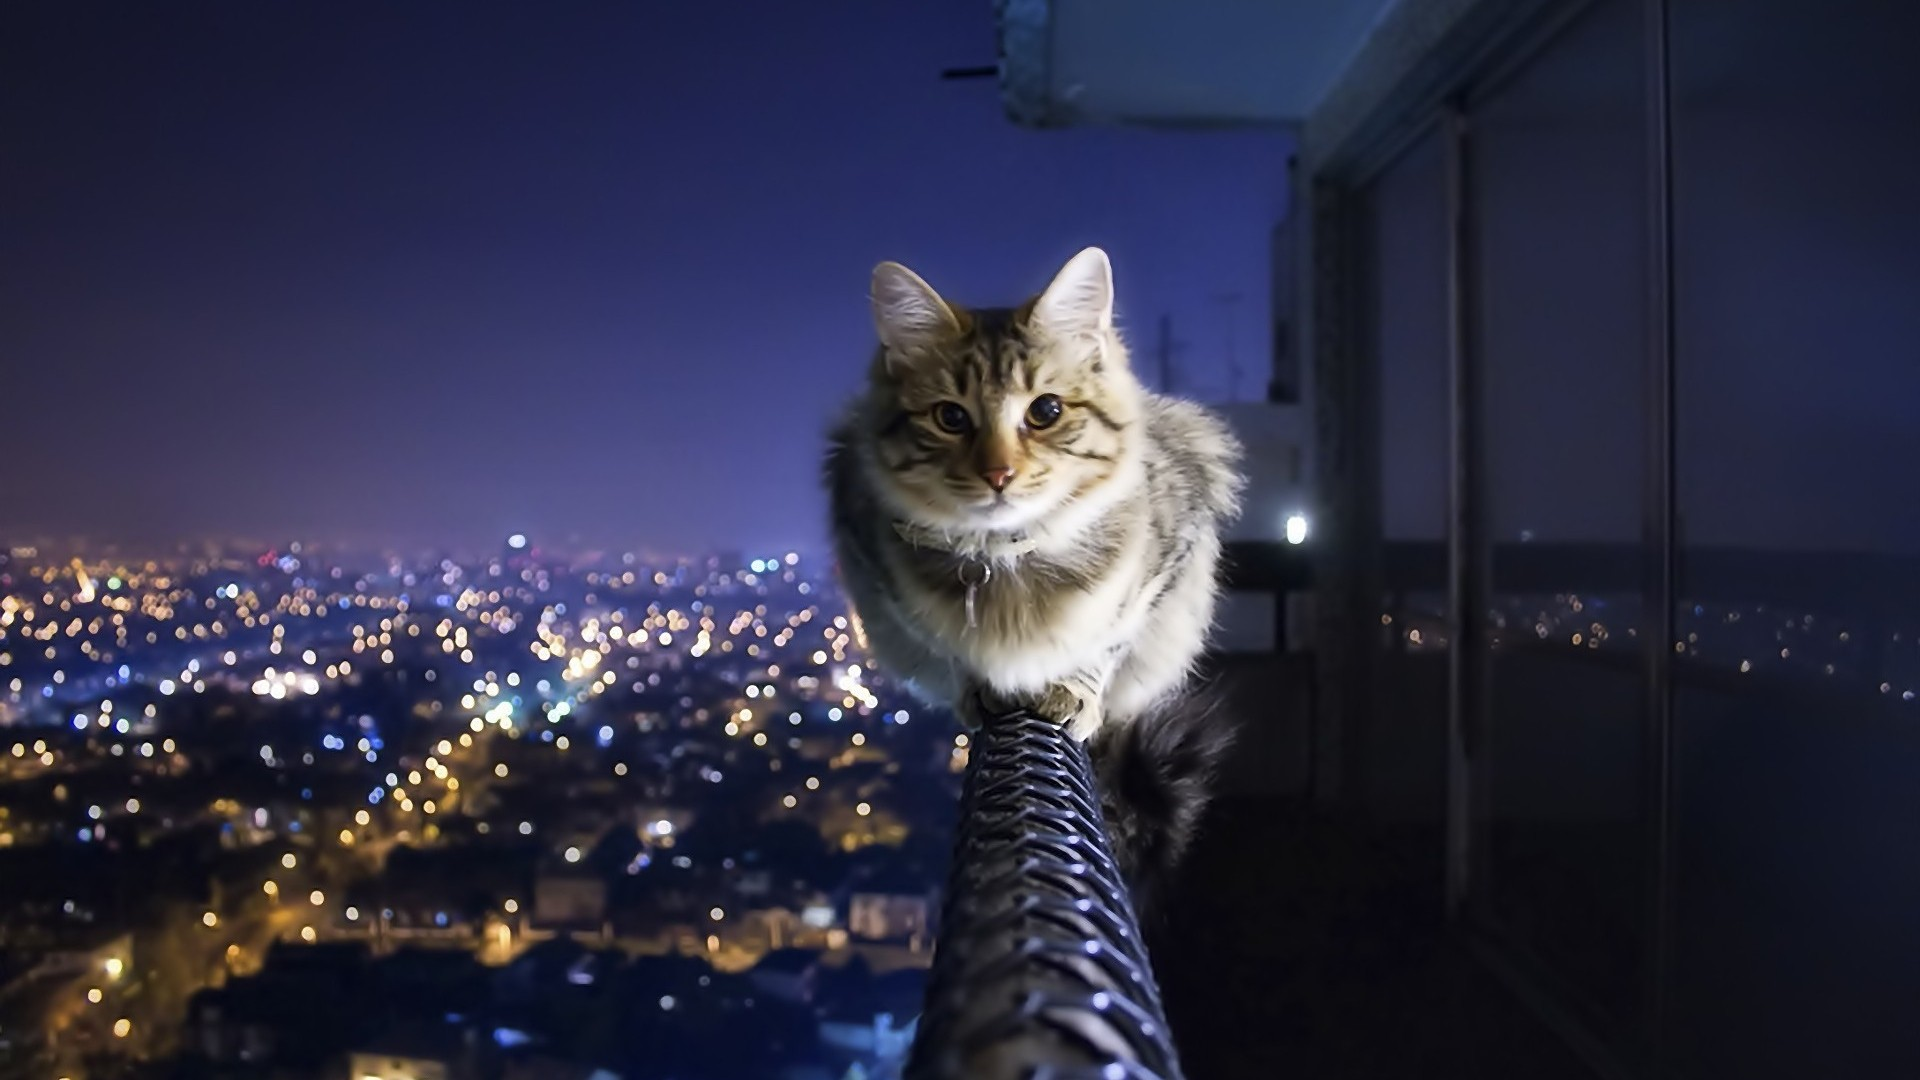
\includegraphics[width=0.50\textwidth]{./Pic/cat.JPG}
% 图片标题
\caption{This is a cat.}
\label{fig:1}       % 给图片一个标签便于交叉引用
\end{figure}

%并列插入图片
\begin{figure}[!h]
  \centering %使得插入的照片居中显示
  \begin{minipage}[t]{.49\linewidth}
   % \framebox{Text}
  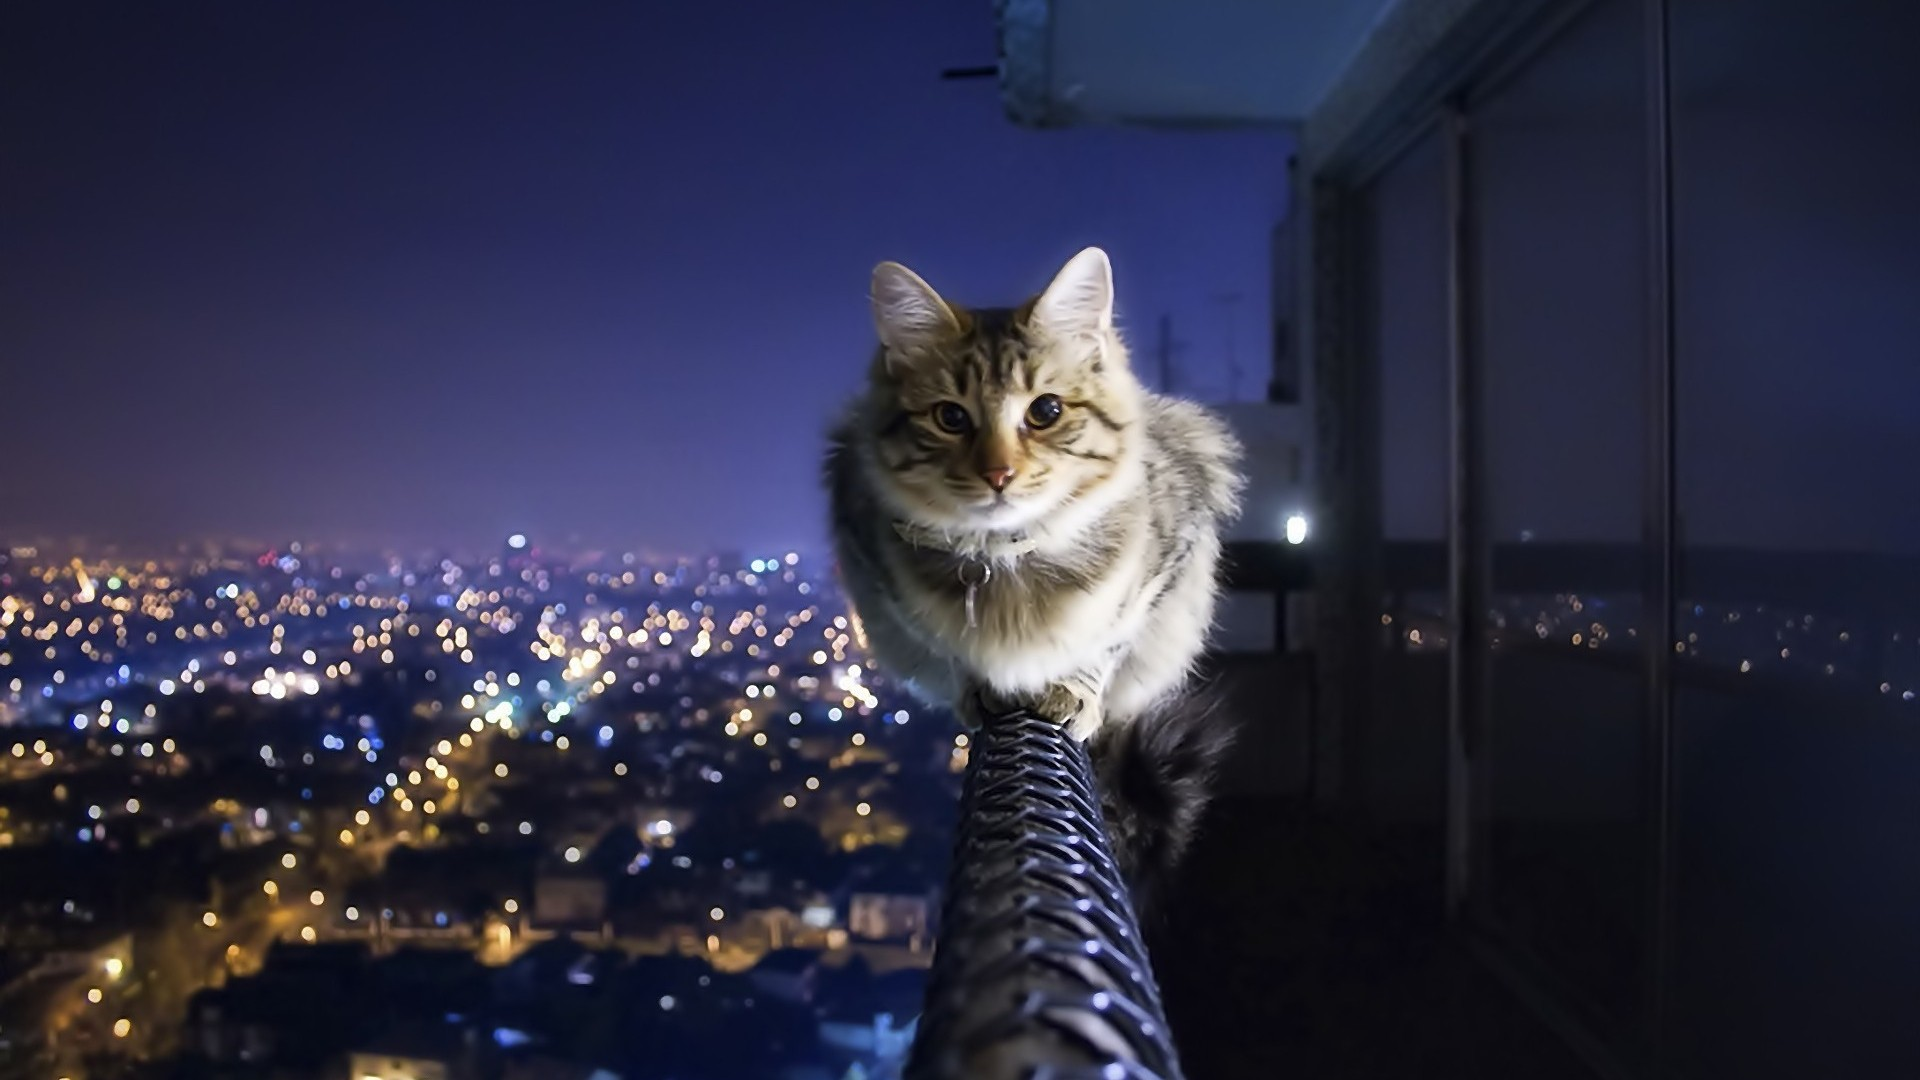
\includegraphics[width=1\textwidth]{./Pic/cat.JPG}
  \caption{This is a cat.}
  \end{minipage}
  \begin{minipage}[t]{.49\linewidth}
  
\includegraphics[width=1\textwidth]{./Pic/human.jpg}
   %\framebox{Text}
  \caption{This is the back of a human.}
  \end{minipage}
\end{figure}

\subsection{Model two:}

\subsubsection{Test insert math formulas}
In the section, we will insert math formulas.\\
%插入文本中的公式\\
\begin{math}\label{math_1} \ln{(x+1)}+\max{\{\varepsilon,\theta\}} \end{math}\\
%居中并编号的公式\\
\begin{equation}\label{eq:eps} \exists~\delta>0,\quad when \quad |x-x_0|<\delta,\quad s.t.~ |f(x)-f(x_0)|<\varepsilon \end{equation}\\
%居中不编号的公式
\begin{displaymath}\label{math_2} \ln{(x+1)}+\max{\{\varepsilon,\theta\}} \end{displaymath}
\[\ln{(x+1)}+\max{\{\varepsilon,\theta\}}\]%简写形式,同上

\subsubsection{Test Equations}%测试方程组
%这个不加左边的大括号,且每个式子都编号了
\begin{eqnarray}
f(x) & = & \cos x \\
f'(x) & = & -\sin x \\
\int_{0}^{x} f(y)dy & = & \sin x
\end{eqnarray}

\subsubsection{Others}
\[
   \begin{aligned}
   A &= (B + C) + D\\
    &=B + (C + D)\\
   \end{aligned}
\]

OK, let's look at another one.
%这个加了左边的大括号,只有一个编号
\begin{equation}
  \left\{
   \begin{aligned}
   \overset{.}x(t) &=A_{ci}x(t)+B_{1ci}w(t)+B_{2ci}u(t)  \\
   z(t) &=C_{ci}x(t)+D_{ci}u(t) \\
   \end{aligned}
   \right.
\end{equation}

 \[
  A = \left(\begin{array}{ccc}
        a_{11} & a_{12} & a_{13} \\
        a_{21} & a_{22} & a_{23} \\
        a_{31} & a_{32} & a_{33}
      \end{array}\right).
  \]

\subsection{Result Analysis:}

%研究人员综合排名
\begin{table}[!h]%[!hptb]
\centering
\caption{Rank of Researcher (Top 10)}\label{Q2:RankTable For Researcher}%便于交叉引用
\begin{tabular}{c l}
    \toprule[2pt]
    \textbf{Rank} & \makecell[c]{\textbf{Researcher Name}}\\
	\midrule[2pt]
    %\hline
	1 & ALON, NOGA M.\\
	2 & HARARY, FRANK*\\
	3 & GRAHAM, RONALD LEWIS\\
	4 & BOLLOBAS, BELA \\
	5 & RODL, VOJTECH\\
	6 & SOS, VERA TURAN\\
	7 & TUZA, ZSOLT\\
	8 & FUREDI, ZOLTAN\\
	9 & SPENCER, JOEL HAROLD\\
	10 & POMERANCE, CARL BERNARD\\
    \bottomrule[2pt]
\end{tabular}
\end{table}

\section{The Influence of Papers}%同理
%表1:研究人员综合排名
\begin{table}
\centering
\caption{Rank of Researchers' Total Influence (Top 10)}%\label{Q2:RankTable For Researcher}% 便于交叉引用
\begin{tabular}{C{3cm} l}
    \toprule[2pt]
    \textbf{Rank} & \makecell[c]{\textbf{Researcher Name}}\\
	\midrule[2pt]
    %\hline
	1 & ALON, NOGA M.\\
	2 & GRAHAM, RONALD LEWIS\\
	3 & RODL, VOJTECH\\
	4 & BOLLOBAS, BELA\\
	5 & HARARY, FRANK*\\
	6 & FUREDI, ZOLTAN\\
	7 & TUZA, ZSOLT\\
	8 & SOS, VERA TURAN\\
	9 & SPENCER, JOEL HAROLD\\
	10 & GYARFAS, ANDRAS\\
    \bottomrule[2pt]
\end{tabular}
\end{table}

\begin{table}[!h]
\centering
\caption{Test}
\begin{tabular}{c | c| >{\columncolor{yellow}}c}
\toprule[1pt]
\diagbox{No.}{Title} & \textbf{L-Title} & \textbf{R-Title}\\
\hline
1 & One & First\\
\cellcolor[rgb]{.9,.9,.9} 2 & Two & Second\\
\cellcolor[rgb]{.2,.9,.9} 3 & Three & Third\\
\bottomrule[1pt]
\end{tabular}
\end{table}

\section{Model Extension}%模型推广

\section{Error/Sensitivity Analysis}%误差/灵敏度分析

\section{Analysis of The Model}% 模型分析


%以下是参考文献
\phantomsection%生成该页的链接
\addcontentsline{toc}{section}{\refname}
\begin{thebibliography}{}
%
% 使用指令\bibitem 构造一条参考文献.
% 具体构造方式,参考以下参考文献格式说明以及示例
% 应尽可能使用英文格式
%
\bibitem{RefJ}
% 期刊引用格式
    % 中文的引用格式
    % 作者. 标题[J].期刊名, 发表年份,  卷号(期号), 页码
    % Author. Article title[J]. Journal name, year, Volume(issue), page numbers.
    % 姓,名字首字母.(年). 题目. 期刊名(斜体), 卷号(期号), 页码.
    Last name, Initials. (year). Title.\emph{The journal name}. Volume(Issue), pages.
    %或者 Last name, Initials.,& Last name, Initials. (year). Title.\emph{The journal name}. Volume(Issue), pages.

\bibitem{RefB}
% 书本/专著引用格式
    % 中文的引用格式
    % 作者名. 书名[M]. 出版地: 出版社, 出版年份: 页码.
    % Author. Book title[M]. Address: Publisher, year: page numbers.
    % 英文引用格式
    % 姓, 名字首字母.(年). 书名(斜体). 出版社所在城市: 出版社.
    Last name, Initials. (year). \emph{Book name}. Address: Publisher.

\bibitem{RefC}
% 文集中的文章
    % 英文引用格式
    % 姓, 名字首字母. (年). 文集名, 文章名(pp.页码). 出版地: 出版社
    Last name, Initials. (year). Collection name, \emph{Article name}(pp.pages). Address: Publisher.

% 学位论文引用格式(英文里等同于专著引用)
\bibitem{RefD}
Author. Article Title[D]. Address: Saver, year: page numbers.
% 网络引用(百科,博客等)
\bibitem{RefI}
The site name, Title. The Site Link. Time.
% 电子文献
\bibitem{RefE}
The main responsibility author. Electronic document titles. Electronic literature source[Symbol]. Site Link, Publish or update date / date references.

% etc
\end{thebibliography}

\begin{appendices}
% 添加多目录
% \include{Appendix1}
% This is Appendix1
% \include{Appendix2}
% This is Appendix2
\section{First appendix}

some text...


Here are simulation programmes we used in our model as follow.\\


\codetitle{Input matlab source:}
\lstinputlisting[language=Matlab]{./code/matlab1.m}


\section{Second appendix}

some more text

\codetitle{Input C++ source:}
\lstinputlisting[language=C++]{./code/sudoku.cpp}
\end{appendices}


\end{document}
